\documentclass[a4paper,11pt]{article}
\usepackage{amsmath,amsthm,amsfonts,amssymb,amscd,amstext,vmargin,graphics,graphicx,tabularx,multicol} \usepackage[french]{babel}
\usepackage[utf8]{inputenc}  
\usepackage[T1]{fontenc} 
\usepackage[T1]{fontenc}
\usepackage{amsmath,amssymb}
\usepackage{pstricks-add,tikz,tkz-tab,variations}
\usepackage[autolanguage,np]{numprint} 

\setmarginsrb{1.5cm}{0.5cm}{1cm}{0.5cm}{0cm}{0cm}{0cm}{0cm} %Gauche, haut, droite, haut
\newcounter{numexo}
\newcommand{\exo}[1]{\stepcounter{numexo}\noindent{\bf Exercice~\thenumexo} : \marginpar{\hfill /#1}}
\reversemarginpar


\newcounter{enumtabi}
\newcounter{enumtaba}
\newcommand{\q}{\stepcounter{enumtabi} \theenumtabi.  }
\newcommand{\qa}{\stepcounter{enumtaba} (\alph{enumtaba}) }
\newcommand{\initq}{\setcounter{enumtabi}{0}}
\newcommand{\initqa}{\setcounter{enumtaba}{0}}

\newcommand{\be}{\begin{enumerate}}
\newcommand{\ee}{\end{enumerate}}
\newcommand{\bi}{\begin{itemize}}
\newcommand{\ei}{\end{itemize}}
\newcommand{\bp}{\begin{pspicture*}}
\newcommand{\ep}{\end{pspicture*}}
\newcommand{\bt}{\begin{tabular}}
\newcommand{\et}{\end{tabular}}
\renewcommand{\tabularxcolumn}[1]{>{\centering}m{#1}} %(colonne m{} centrée, au lieu de p par défault) 
\newcommand{\tnl}{\tabularnewline}

\newcommand{\trait}{\noindent \rule{\linewidth}{0.2mm}}
\newcommand{\hs}[1]{\hspace{#1}}
\newcommand{\vs}[1]{\vspace{#1}}

\newcommand{\N}{\mathbb{N}}
\newcommand{\Z}{\mathbb{Z}}
\newcommand{\R}{\mathbb{R}}
\newcommand{\C}{\mathbb{C}}
\newcommand{\Dcal}{\mathcal{D}}
\newcommand{\Ccal}{\mathcal{C}}
\newcommand{\mc}{\mathcal}

\newcommand{\vect}[1]{\overrightarrow{#1}}
\newcommand{\ds}{\displaystyle}
\newcommand{\eq}{\quad \Leftrightarrow \quad}
\newcommand{\vecti}{\vec{\imath}}
\newcommand{\vectj}{\vec{\jmath}}
\newcommand{\Oij}{(O;\vec{\imath}, \vec{\jmath})}
\newcommand{\OIJ}{(O;I,J)}

\newcommand{\bmul}[1]{\begin{multicols}{#1}}
\newcommand{\emul}{\end{multicols}}


\newcommand{\reponse}[1][1]{%
\multido{}{#1}{\makebox[\linewidth]{\rule[0pt]{0pt}{20pt}\dotfill}
}}

\newcommand{\titre}[5] 
% #1: titre #2: haut gauche #3: bas gauche #4: haut droite #5: bas droite
{
\noindent #2 \hfill #4 \\
#3 \hfill #5

\vspace{-1.6cm}

\begin{center}\rule{6cm}{0.5mm}\end{center}
\vspace{0.2cm}
\begin{center}{\large{\textbf{#1}}}\end{center}
\begin{center}\rule{6cm}{0.5mm}\end{center}
}



\begin{document}
\pagestyle{empty}
\titre{Contrôle 2 : Nombres relatifs, droites remarquables et centre de symétrie }{Nom :}{Prénom :}{Classe}{Date}



\exo{3,5} 

\q Comparer :  

- 4  . . . .  9\hfill  /\hfill 408,3 . . . . 480,3 \hfill/\hfill  - 5,001 . . . .  - 5,01\hfill /\hfill  - 34,04 . . . . 0 \hfill/\hfill 9,03 . . . .  - 9,03\hfill/ \hfill - 5,7  . . . .  - 5,8\\

\q Quel est le plus grand entier relatif inférieur à (+ 17,25) ?\\
Quel est le plus petit entier relatif supérieur à (– 36,75)?\\


\exo{2} (\textbf{Sur le sujet})

\initq \q  Placer les points A et B d'abscisses respectives (+ 7) et (– 1). Les marquer d'une croix bleue.\\

\includegraphics[scale=1]{Abscisses1.eps} 

\q Placer le point C d'abscisse  (+ 2) et le point D d'abscisse  (– 14). Les marquer d'une croix bleue.\\


\includegraphics[scale=1]{Abscisses2.eps} 

\exo{4,5} (\textbf{sur le sujet sauf la question 1)} )

\initq \q Donner les coordonnées des points A, C, E et D.\\

\q Placer en les marquant d'une croix bleue, les points :	K ( 0 ; 1,5)	et	L ( – 1,25 ; 0 ).\\	

\q  Le point B a la même abscisse que A et la même ordonnée que  C. Le point P a la même abscisse que C et la même ordonnée que A. Placer les points B et P.\\

\q Colorier en vert les points dont l'abscisse est – 3.\\

\includegraphics[scale=1]{coordonnees.eps} \\

\exo{3}\\

\initq \q Tracer un triangle ABC tel que AB = 4 cm, AC = 5,5 cm et BC = 6 cm.\\

\q Tracer en vert la hauteur issue de A et en bleu la hauteur issue de C.\\

\q Nommer H le point d'intersection de vos 2 hauteurs précédentes. Comment s'appelle ce point ?\\

\q Que peut-on dire des droites (BH) et (AC) ? \textbf{Justifier.}\\


\exo{1,5} Pour chaque question entourée la bonne réponse. (\textbf{Sur le sujet})\\

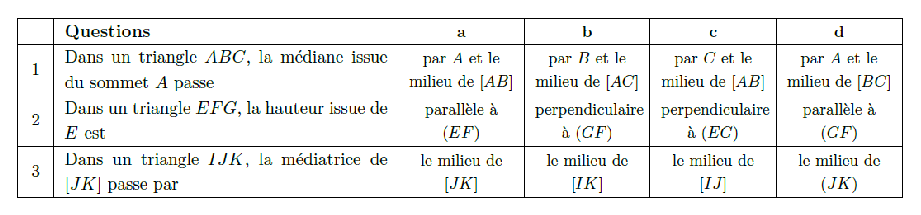
\includegraphics[scale=1]{qcm.eps} \\



\exo{2}(\textbf{Sur le sujet})
\bmul{2}

\begin{flushleft}
\includegraphics[scale=0.83]{epee.eps} 
\end{flushleft}

\columnbreak

L'épée magique du Roi Arthur, Excalibur (E), a été cachée. 
Retrouver l'emplacement de sa cachette sur le plan ci-dessous, sachant que :\\

- elle est à égale distance du château C et du lac au dragon L ;\\

- elle est sur la hauteur relative au côté [TL] dans le triangle CTL.\\

Laisser les traits de construction.\\

\emul


\exo{1,5} (\textbf{Sur le sujet}) Tracer le cercle circonscrit au triangle RSE ci-dessous. Laisser tous les traits de construction.\\

\includegraphics[scale=1]{cerclecirconscirt.eps} \\


\exo{2} (\textbf{sur le sujet}) Trouve le centre de symétrie lorsqu'il existe des figures ci-dessous. Trace le en \underline {bleu}.


\includegraphics[scale=0.9]{centresym.eps} 
\includegraphics[scale=1.2]{centresym2.eps} 
\includegraphics[scale=1.1]{centresym3.eps} 

\end{document}
